\chapter{Results}
This part of the Master's Thesis will run the simulation models and compare the results of different option valuation methods. Furthermore, a sensitivity analysis will be performed to determine the influence of some of the parameters used in the models.

Due to the large amount of routes, only interesting or surprising results will be displayed and analysed in this chapter. Full tables with results can be found in the appendices \todo{ref}.


\section{Simulation 1: the all knowing seller}
First, the simulation will be configuration to simulate an all knowing seller with foreknowledge. The specific arrangement and description of its parameters can be found in \typenameref{chap:ModelDevelopment}. A summary of the level of the parameters can be found in \autoref{tbl:ParameterConfigAllKnowingSeller}.


\begin{table}
\begin{center}
\begin{tabular}{l l c r}
    \toprule
    \#  & Parameter  &  Symbol  &  Level \\
    \midrule
    1  &  option's days till maturity  &  $m$  & 3~days \\
    2  &  option's strike price  &  $p_S$  &  $p_I$  \\
    3  &  seller's forecasting technique  &  ~  & foreknowledge \\
    4  &  passenger's risk parameter  &  $\mbox{RP}$  &  0.1 \\ 
    5  &  passenger's forecasting technique  &  ~  &  historical data \\
    6  &  passenger's likelihood of travelling  &  $P^f$  &  0.5 \\
    7  &  arrival rate of passengers  &  ~  &  $(42 - m)$ per flight \\
    8  &  simulation's number of trials  &  $N$  &  150 \\
    \bottomrule
\end{tabular}
\caption{Parameters for the all knowing seller with foreknowledge}
\label{tbl:ParameterConfigAllKnowingSeller}
\end{center}
\end{table}


Furthermore, three assumptions are being made during the simulation of this model, namely:
\begin{compactenum}
\item the option's maximum price shall not exceed 15~percent of the current ticket price;
\item the seller knows in advance whether the customer will exercise its option;
\item the seller knows the exact level of the customer's Willingness to Pay.
\end{compactenum}


The combination of parameter and assumption number~2 is what identifies this simulation model. The seller uses foreknowledge and thus has the ability to forecast prices at maturity with a hundred~percent accuracy. Therefore, the risk of prediction errors has been eliminated. Furthermore, assumption~2 gives the seller \emph{all knowing} information on which he can act consequently. As an example, consider the seller thus already knows at the time when he offers the option that the passenger is \emph{not} going to exercise its option at maturity. He can therefore offer his option at any price higher than 0, as he is sure the passenger will not cost him anything at the time of maturity. The option writing company will thus sell an option to all the passengers with a WTP greater than 0. On the other hand, when the seller sees beforehand that the passenger \emph{does} exercise his option, his Willingness To Accept will equal his expected losses from offering the option (i.e., $p_{t+m} - p_t$). In this case the option writer will only offer options to passengers with a WTP greater than his WTA.

Because of this combination of parameters and assumptions, the option seller will be able to set the prices of options at the most optimal level. The seller will therefore be able to set the most optimum prices and gain maximum possible profits.

This first simulation model will create an understanding on these maximum profits and optimal level of sales for the dataset. Furthermore, because uncertainties and risks of unavailable information have been eliminated, sensitivity analysis will also be performed. This sensitivity analysis will shed light on the influence of some of the parameters used in this section.


\subsection{Analysis of the results}
\label{subsec:AnalysisOfAllKnowing}
The simulation was first run on all the different routes using the parameters defined in previous section. The results of the simulations can be found in \autoref{tbl:resultsAllKnowing} of \autoref{app:SimulationResultsAllKnowingSeller}.

The column labelled \emph{Ticket} contains the mean ticket price of that particular route. The two columns next to that shows the average price of airfare~lock-in products which are actually sold to the passengers. The first gives the absolute values, and the latter displays the price relative to the mean ticket price. The columns labelled \emph{Option profits} show the mean profits made on these sold options. Again, the first value is absolute, while the second is relative to the mean option price. The final column shows the percentage of options sold relative to the total options offered. The total number of options sold is given by parameter~6.

As is shown in the table, the option prices range on average from about 2~percent of the mean ticket price, up till almost 10~percent. This seems to be in alignment with the empirical airfare~lock-in product prices seen at some airliner's websites. However, one should note that the option seller in this specific simulation only offers options to passengers of which the writer is certain of a positive return. This is also implied by the high profit percentages. These were acquired due to the writer information on which passengers will exercise the option, in which the seller could handle accordingly for each specific situation.

The difference of relative options prices between routes can not directly be explained by the results found in the table. This could have been caused by the forecasting accuracy of the passenger, because most of the other factors were static amongst the different routes. To test this, first the forecasting accuracy of the customer per route had to be quantified. In this research I have chosen to use the mean absolute percentage error ($\mbox{MAPE}$), which is defined as:

$$\mbox{MAPE} = \frac{1}{42}\sum_{t=1}^{42} \left| \frac{p_{t+1}-p_t}{p_{t+1}}\right|$$

Next, Pearson's correlation, $\rho$, of the route-specific $\mbox{MAPE}$s and relative option prices was computed. The result of this test can be found in \autoref{tbl:pearsonPricesMAPE}. The statistical test clearly shows a positive and significant correlation between both variables. The combinations of the observed relative option prices and passenger's $\mbox{MAPE}$ have been plotted in \autoref{fig:optionPricesMAPE}. This figure also shows the OLS-regression line.

Both analyses show a positive relation between the passenger's forecasting error, and the relative option prices. This thus implies that when there are more uncertainties in the price, a seller can likely gain from the situation. This, however, was to be expected from the assumption in this simulation model in which the seller knows the customer's maximum Willingness To Pay. A higher $\mbox{MAPE}$ would therefore automatically result in either much to low predictions, or much to high forecasts of ticket prices. The first case would result in a lower number of options sold, as the seller's Willingness To Accept would probably be higher than the customer's WTP. The second case would result in higher relative option prices, as the WTP is likely much higher than the seller's WTA. This also seems to be the case in this simulation.

\todo[implications for real world setting?]{here}


\begin{table}
\centering
\begin{tabular}{l c c}
\toprule
~  &  $\rho_{X,Y}$  &  p-value   \\
\midrule
Pearson's correlation test &  0.7627  &  $< 0.001$ \\
\bottomrule
\end{tabular}
\caption{Correlation of option prices and passenger's $\mbox{MAPE}$}
\label{tbl:pearsonPricesMAPE}
\end{table}


\begin{figure*}
    \centering
    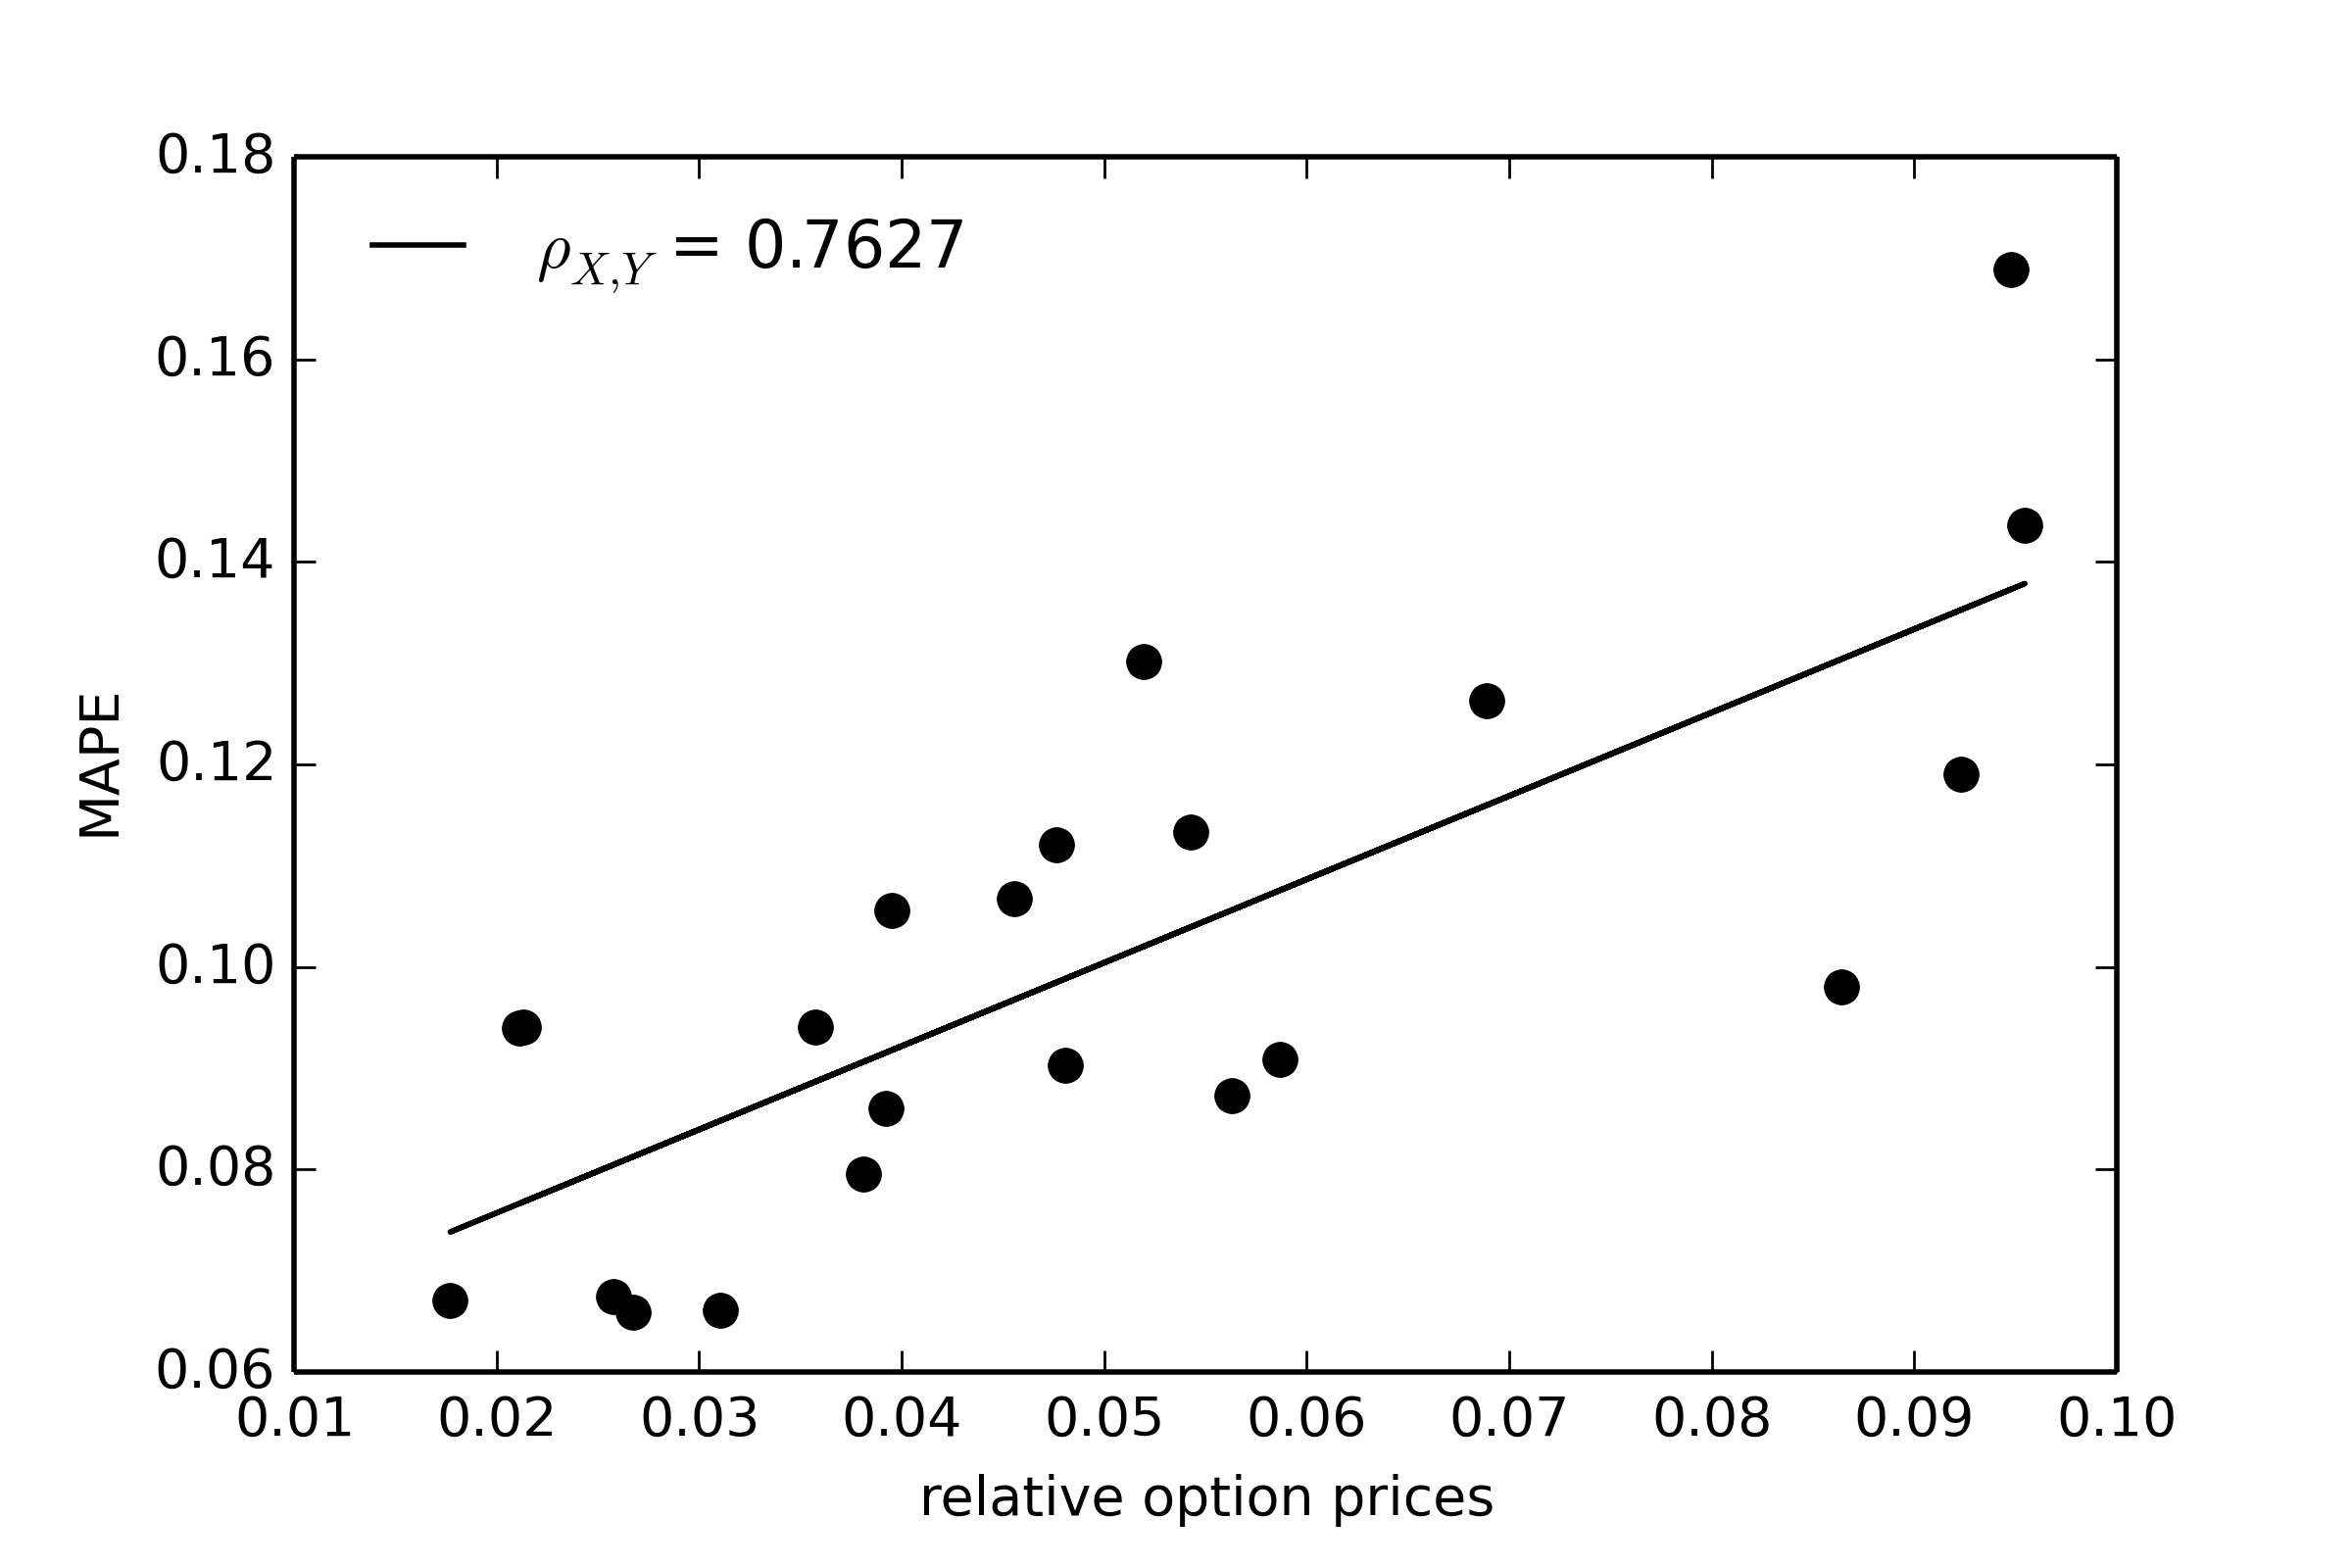
\includegraphics[width=0.8\textwidth]{figures/correlation_optionPrices-MAPE}
    \caption{Correlation between relative option prices and $\mbox{MAPE}$}
    \label{fig:optionPricesMAPE}
\end{figure*}


Next to categorization of the results per route, another insightful display of these values is relative to their number of days before departure. \autoref{fig:OptionPricesDBB} shows the relative options price, as well as the percentage sold to their corresponding days before flight. In this analysis all routes have been aggregated. The left figure shows the results with the assumption that a passenger will never pay more than 15~percent of an option price. The right plot shows the outcomes when this assumption is released.

One will immediately notice that the peaks seen in \autoref{fig:4-plot} of chapter \autoref{chap:DataAnalysis} can also be observed in the graphs. This is as expected, because higher expected price fluctuations automatically yield a higher WTA of the seller and WTP of the passenger.

That the peaks do not exceed above the 16~percent level in the left figure has to do with the assumption made in this research that option prices should never exceed the fifteen~percent level. This also explains the high drop of percentage~sold at about 7~days before departure. In that situation, the seller knew the passenger was going to exercise his option, and that the ticket price was going to increase with more that 15~percent. The seller thus decides to not offer the option, as this will always result in losses.

In the right figure this assumption has been released, which resulted in very high peaks of up to 50~percent of the mean option price. The high increase was also anticipated by the customer's WTP, as the percentage~sold-curve follows a similar pattern. Because it is unlikely a passenger will purchase options for such a high price, the assumption that limits the price at a maximum of 15~percent is applied throughout the rest of this thesis.


\begin{figure}
\centering
\subfloat[][with limits]{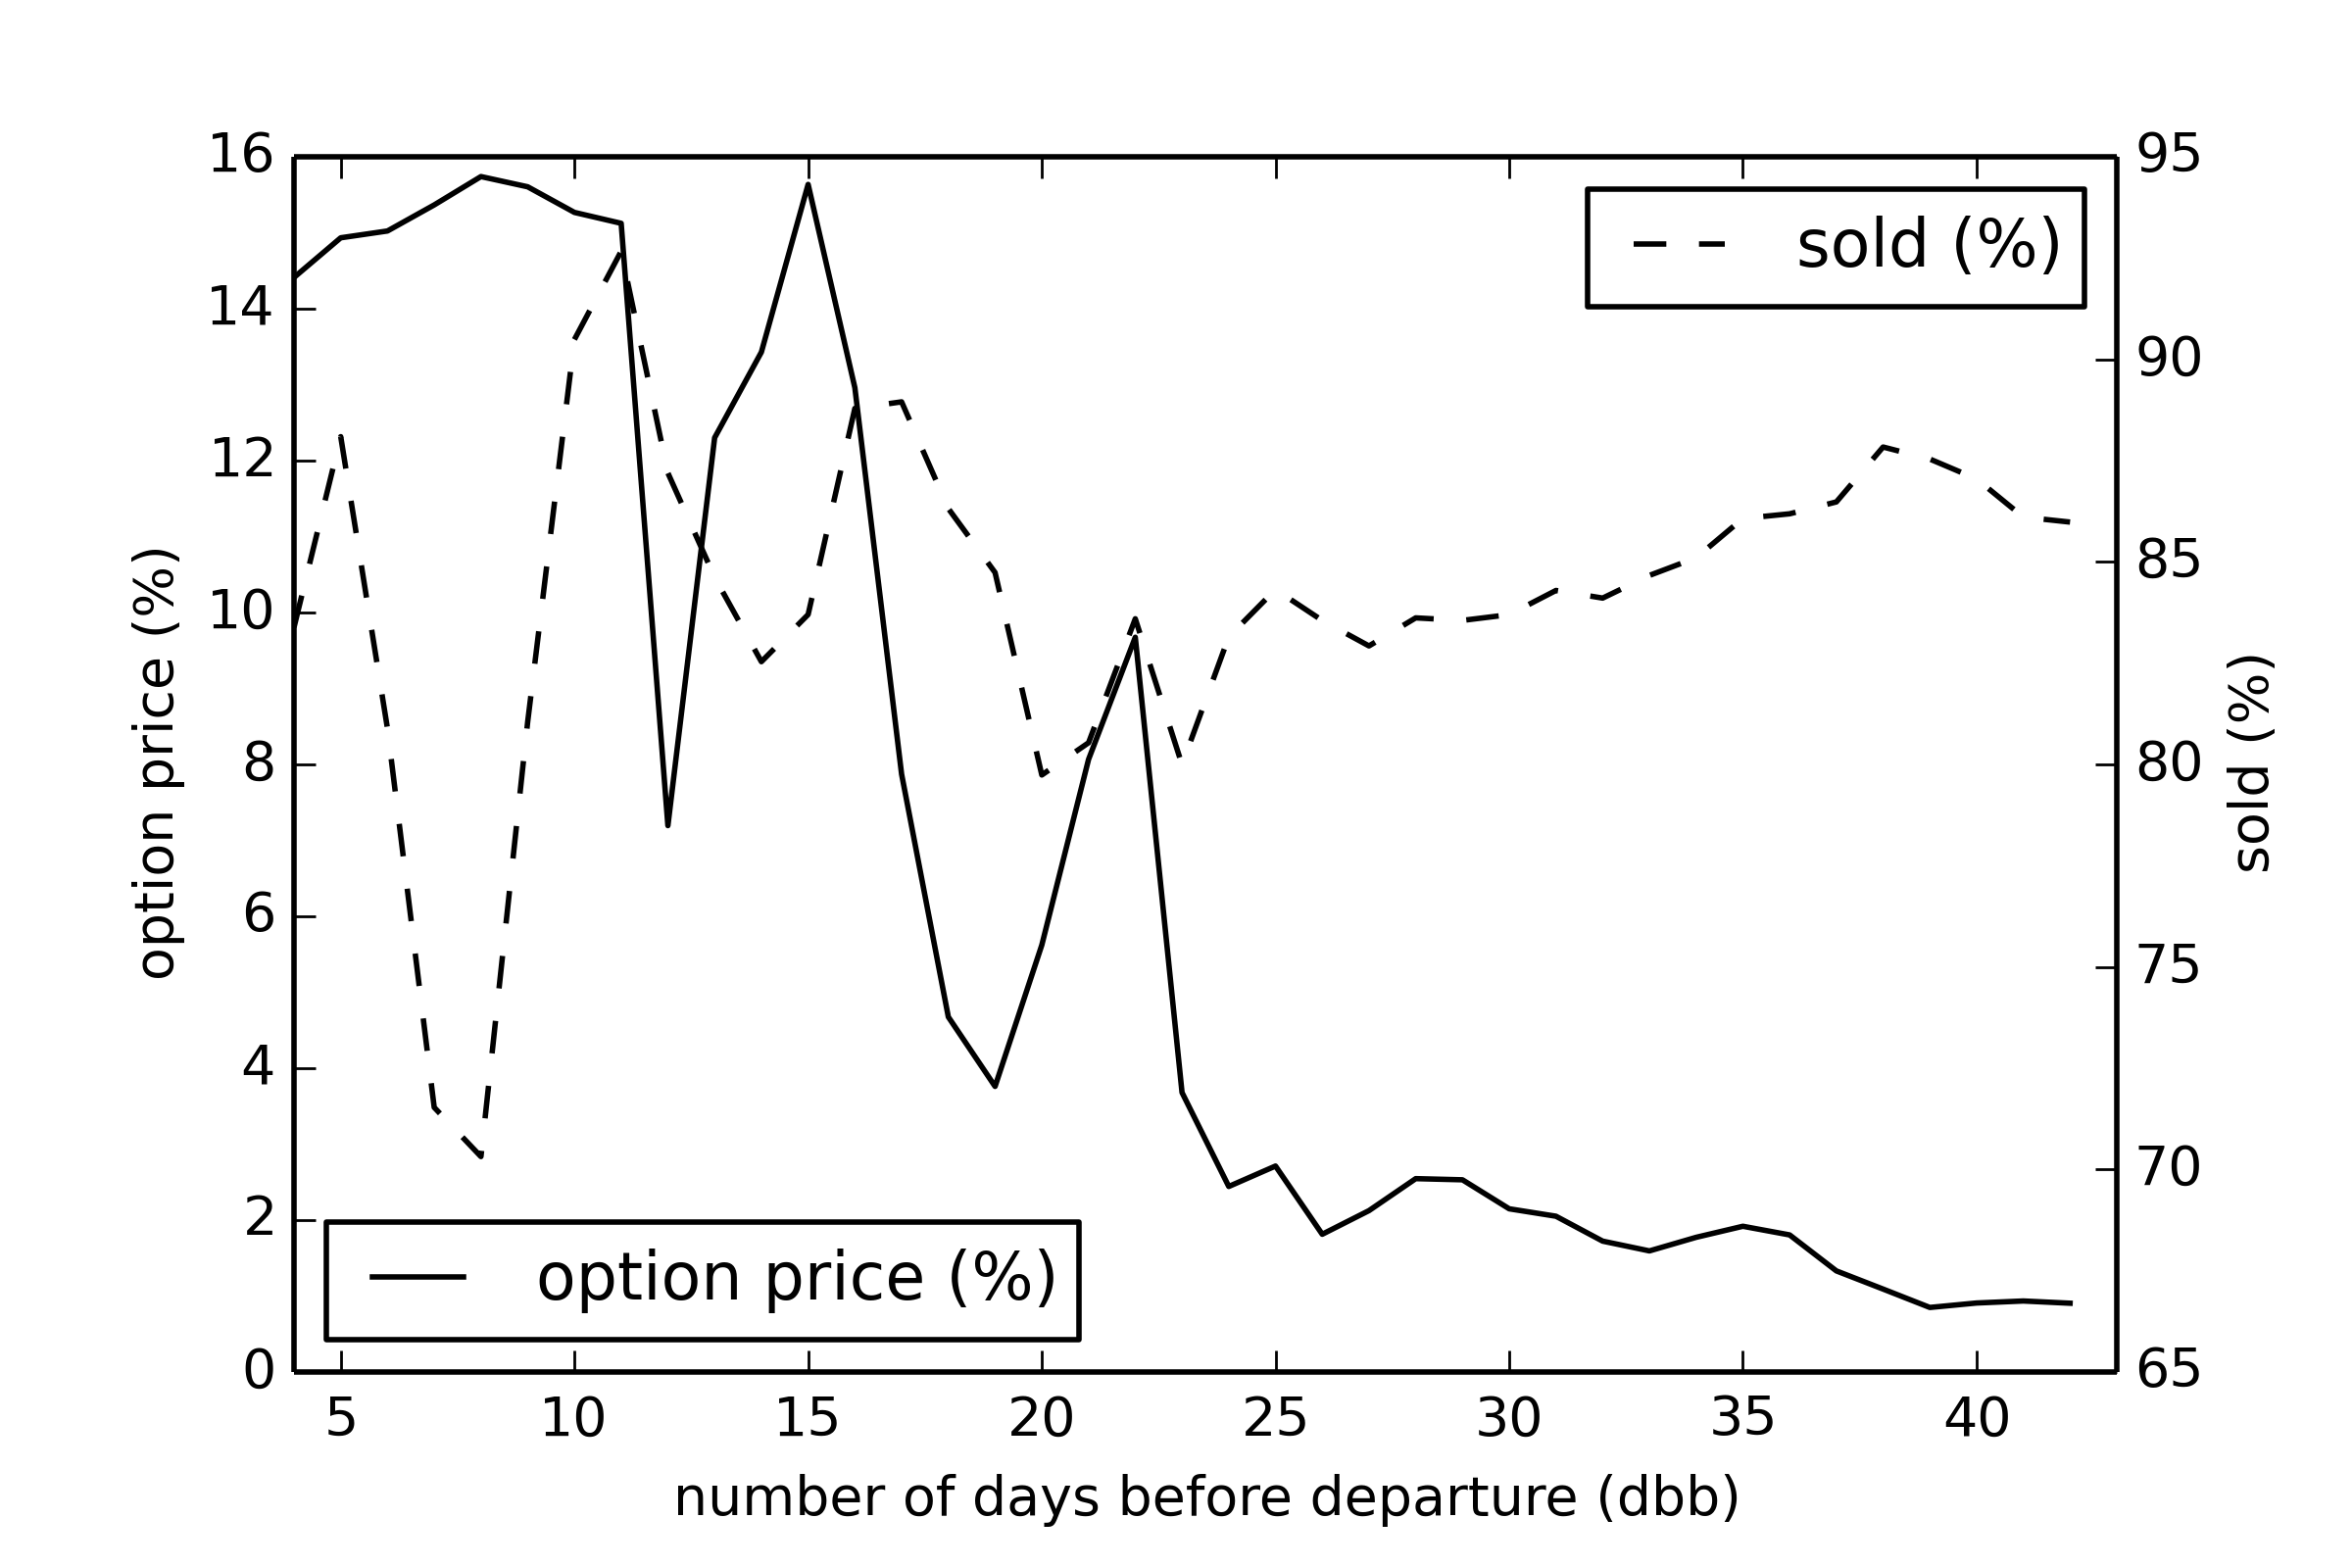
\includegraphics[width=.45\textwidth]{figures/OptionPricesDBB}
}
\qquad
\subfloat[][without limits]{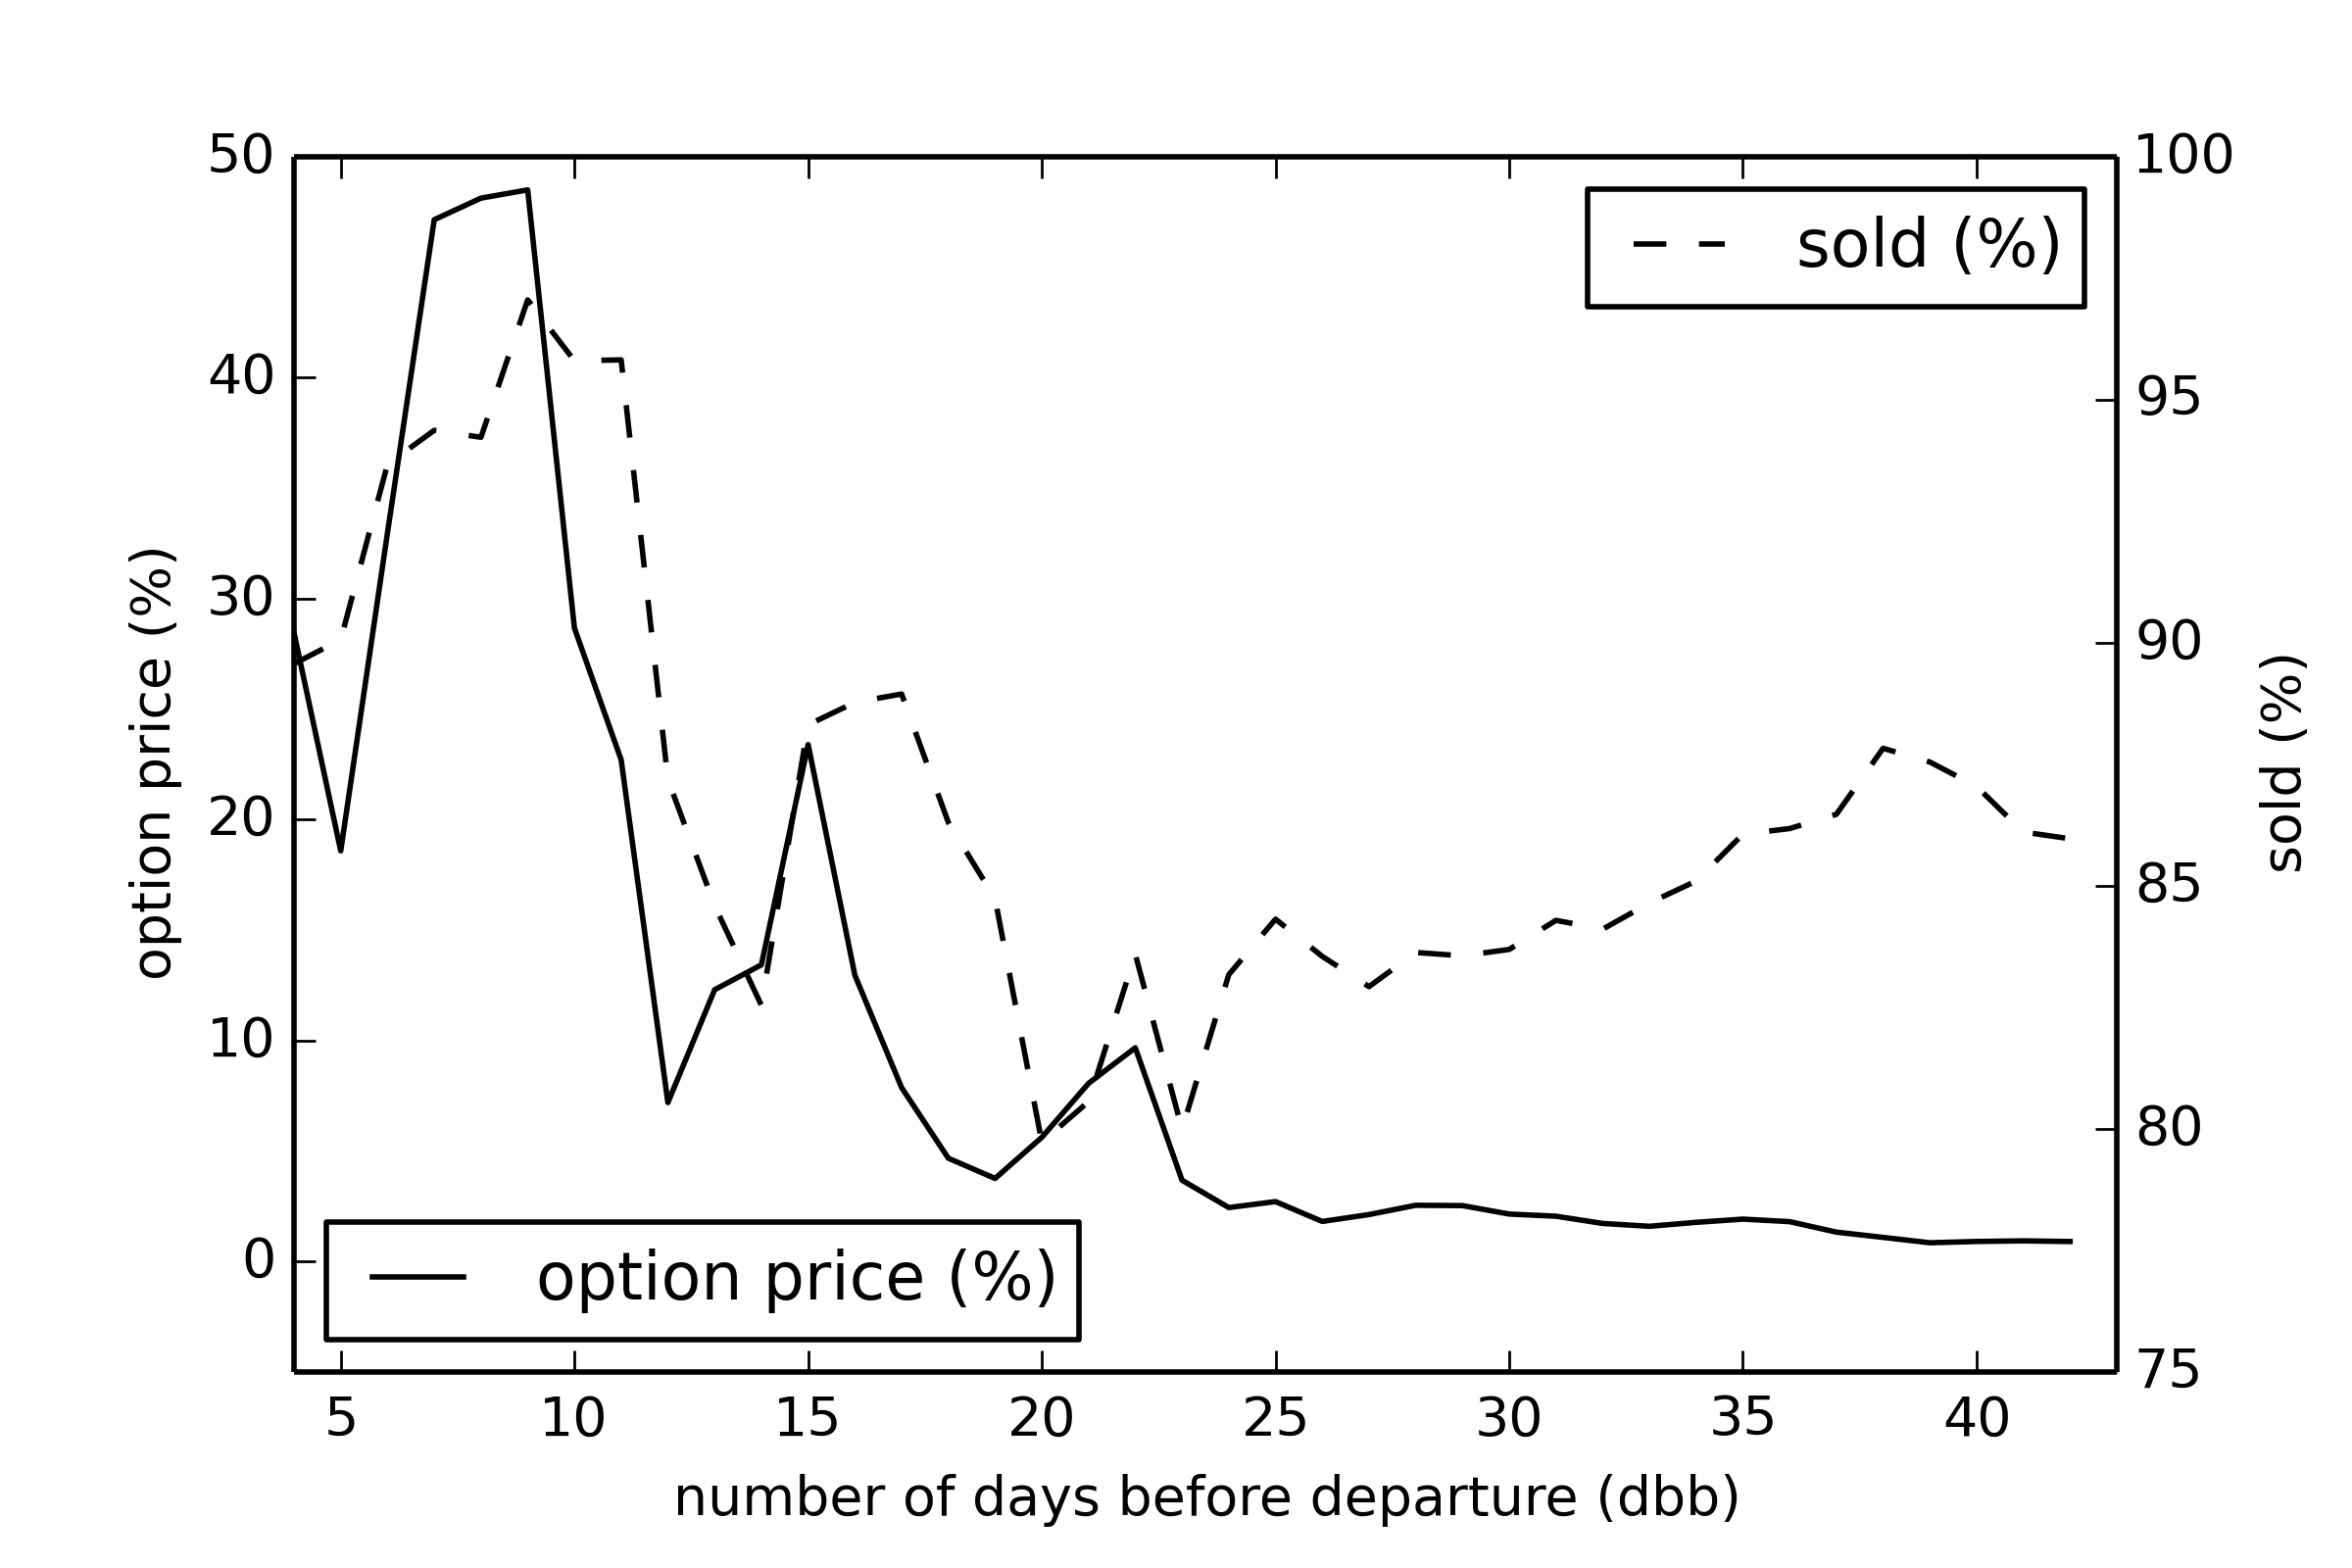
\includegraphics[width=.45\textwidth]{figures/OptionPricesDBB_nolimit}}
\caption{Results relative to number of days before departure}
\label{fig:OptionPricesDBB}
\end{figure}


The results acquired from this simulation model can be interpreted as the maximum profits possible in the current situation. Next section will alter some of the parameters and ascertain their influence on the gains the all knowing seller can receive.


\subsection{Sensitivity analysis}
After the first simulation, a sensitivity analysis is performed. For the base scenario, the all knowing option seller with foreknowledge will still be used. During the analysis only one of the parameters will be adjusted at a time. This way the exact effects of the variable can be examined.

The parameters for which a sensitivity analysis will be performed are \begin{inparaenum}[\itshape (i)\upshape]
    \item the options number of days till maturity,
    \item the passenger's risk parameter, and
    \item the passenger's likelihood of travelling.
\end{inparaenum}

\subsubsection{Option's number of days till maturity}
The first parameter for which a sensitivity analysis is performed is the number of days till maturity, $m$. In the base case, $m$ was set to 3~days, but this number will now be altered to values ranging from a 1~day till 21~days.

I expect the parameter $m$ to be of big influence on the realised profits of the option selling company. This is because the passenger is likely to make less accurate predictions because of the increasing time horizon. On the other hand, however, the option seller in this simulation still has foreknowledge. So, he does not have these increased uncertainties. This will likely create larger gaps between the passenger's WTP and the seller's WTA. Because the assumption is made that the seller knows the passenger's maximum WTP, he will be able to set higher option prices.

Next to this higher expected forecasting error, the option prices will also increase relative to its number of days till maturity, because of the higher probability of a big upward price motion.

Due to the assumption stating that the maximum price will not exceed 15~percent of the current ticket price, I also expect that the values are nearing a limit when $m$ represents more number of days. The curve will thus likely follow a logarithmic function:
$$ y = a + b \ln(m) $$

The percentage of options sold will likely also decrease due to this assumption. The seller with foreknowledge will never actually sell anything below his WTA, but the limit restrains the seller from setting a higher option price.

To compute the outcomes of the sensitivity analysis, the simulation was run on the complete set with all of the routes aggregated. At each run all the variables except the number of days till maturity, $m$, stayed fixed. The variable $m$ was altered to represent values between 1~and 21~days. \autoref{fig:OptionPricesMaturity} shows the sensitivity analysis of the number of days till maturity on the option price and percentage sold. 


\begin{figure*}
    \centering
    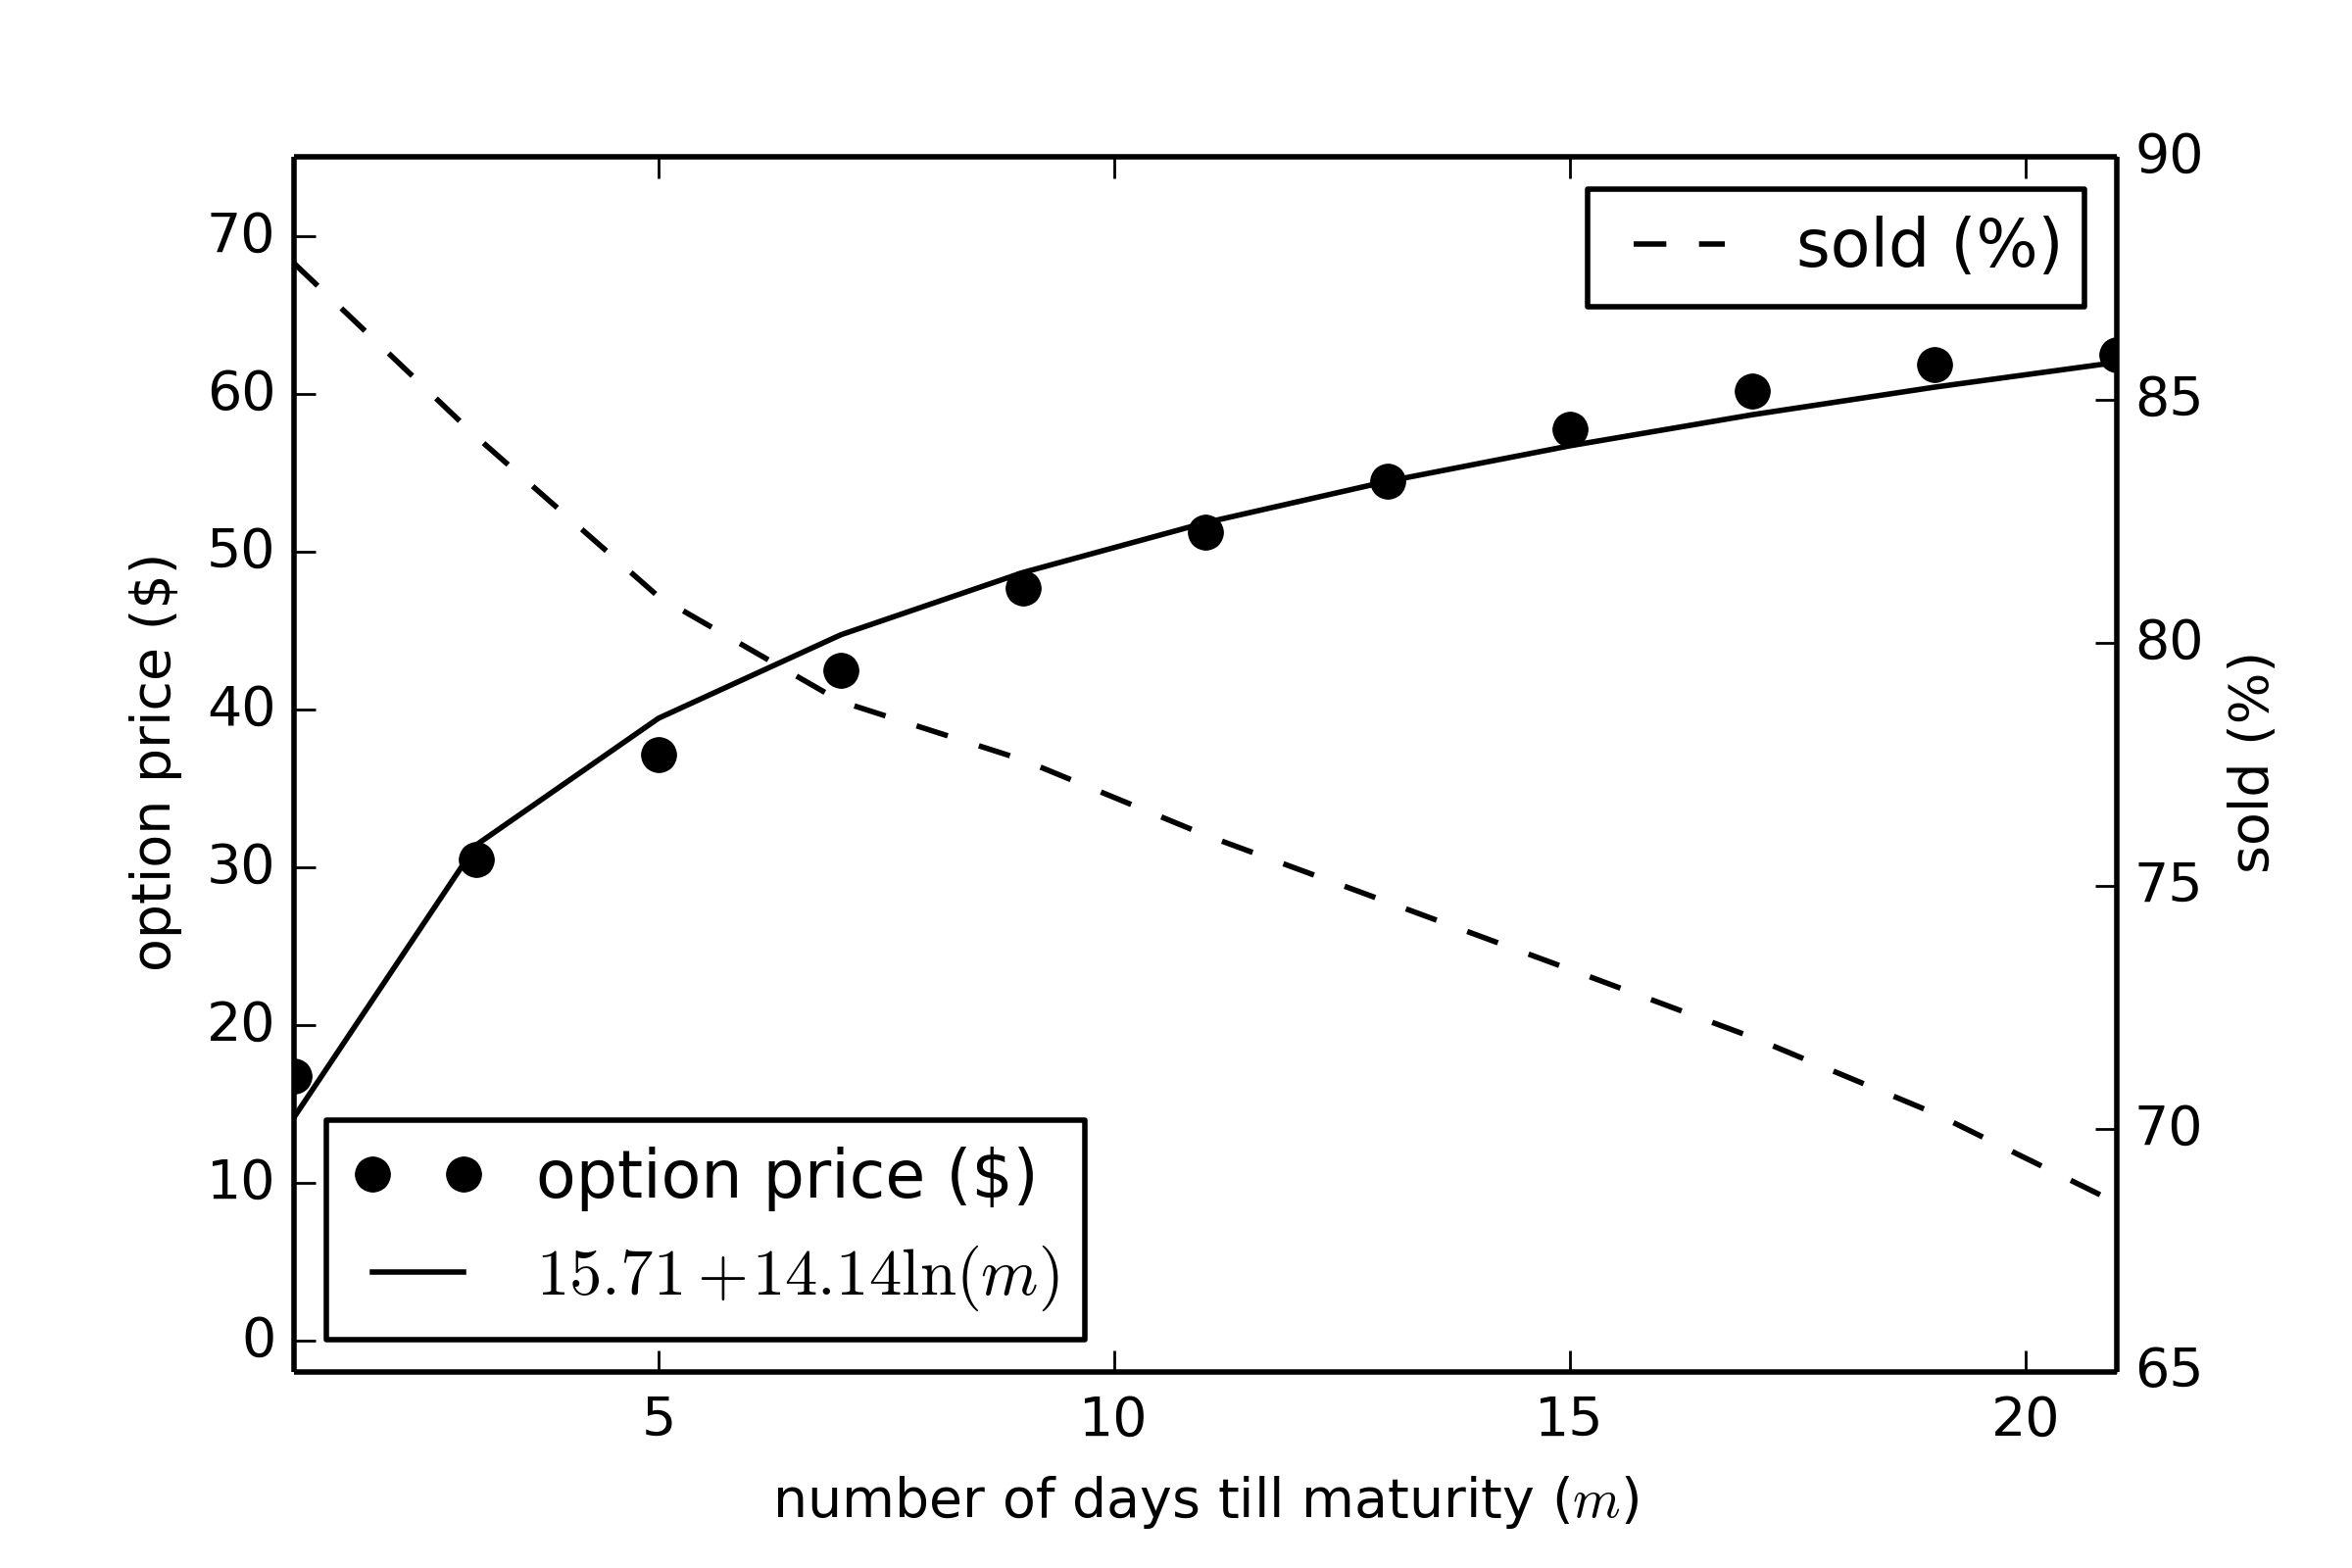
\includegraphics[width=0.8\textwidth]{figures/OptionPricesMaturity}
    \caption{Influence of number of days till maturity ($m$)}
    \label{fig:OptionPricesMaturity}
\end{figure*}


As expected, the absolute option price increases as $m$ increases. The assumed maximum price is also clearly observable in the results. To compute the influence of the variable on the average option price, the observations were fitted on the logarithmic function using the non-linear least square method. Results of this regression are available in \autoref{tbl:FitMaturity}.

The results show a very high correlation between the logarithmic function and the actual observed values. This is enforced by \autoref{fig:OptionPricesMaturity}, which also shows that the observations lie very close to the theoretical line.


\begin{table}
\centering
\begin{tabular}{l c c c c}
\toprule
~  &  $a$  &  $b$  &  $\rho_{X,Y}$  & p-value  \\
\midrule
$y = a + b \ln(m)$  &  15.71  &  14.14  &  0.9941  &  $< 0.001$ \\
\bottomrule
\end{tabular}
\caption{Fitting observations to logarithmic function}
\label{tbl:FitMaturity}
\end{table}


Lastly, the percentage of options sold is also linearly related to the number of days to maturity.

The sensitivity analysis in this sections shows that the variable $m$ has a significant influence on the results gained from the analysis. A logarithmic function had a near-perfect fit with the observed absolute option prices.

Further simulations in this research will set the value $m$ at a level of 3~days. This because this level of $m$ has already been observed in airliners that offer airfare~lock-in products, and it limits the influence of the assumption regarding the maximum option price.


\subsubsection{Passenger's risk parameter}
This section will perform sensitivity analysis on the passenger's risk parameter, $\mbox{RP}$. The variable can be defined as the percentage a passenger is willing to pay extra to get a fixed price in the theoretical situation specified in \autoref{sec:SimulationModel}.

In this sensitivity analysis, the passenger's risk parameter will hold values between 0~and 15~percent. A $\mbox{RP}$ of zero represents a risk~neutral customer. By setting the lower limit to this value, only include risk~neutral and averse persons will be included in the analysis. Passengers with a risk~seeking utilization will not buy options, as they will rather wait instead of buying an airfare~lock-in product or flight ticket immediately. The upper bound is set equal to the assumed maximum option price a customer is willing to pay: 15~percent.

An increase in the risk parameter, $\mbox{RP}$, will results in a steeper risk~aversion curve. This risk~utility function is closely related to the passenger's WTP, as he will be willing to pay more to eliminate the risk of fare fluctuations. Therefore, a higher will level of $\mbox{RP}$ will likely results in higher relative option prices. Furthermore, an increase will probably result in a higher percentage of options sold to passengers, as it is more likely the customer's WTP is exceeding the option writer's WTA.

\autoref{fig:OptionPriceRP} shows the results of the sensitivity analysis on the risk parameter. As clearly can be seen in the plot, both the relative option price and percentage of products sold seem to follow a positive linear trend.

\begin{figure*}
    \centering
    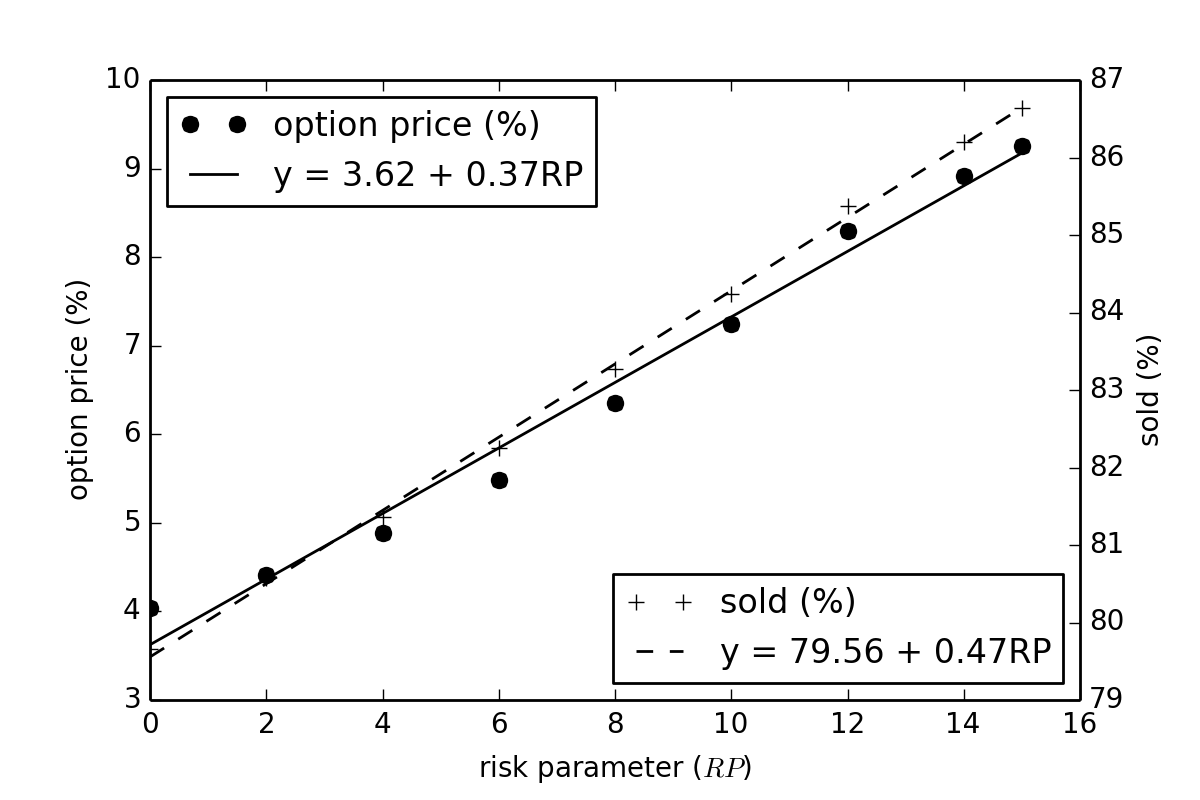
\includegraphics[width=0.8\textwidth]{figures/OptionPrice_RP.png}
    \caption{Influence of the risk parameter ($\mbox{RP}$)}
    \label{fig:OptionPriceRP}
\end{figure*}

Next, the quantitative influence of a change in $\mbox{RP}$ had to be determined. To do so, regression analysis on both the observed values of the relative option prices and percentage sold was performed. The ordinary least squares method was used to find the functions linear parameter. The outcomes are found in \autoref{tbl:FitRP}.

\begin{table}
\centering
\begin{tabular}{l c c c c}
\toprule
~  &  $a$  &  $b$  &  $\rho_{X,Y}$  & p-value  \\
\midrule
Option price (\%)  &  3.62   &  0.37  &  0.9922  &  $< 0.001$ \\
Options sold (\%)  &  79.56  &  0.47  &  0.9943  &  $< 0.001$ \\
\bottomrule
\end{tabular}
\caption{Fitting observations to linear function ($y = a + b \times \mbox{RP}$)}
\label{tbl:FitRP}
\end{table}


As can be seen from the results, both variables are influenced significantly by a change in the risk parameter. Every 1~percent increase in $\mbox{RP}$ results in a 0.37~percent of the relative option price. The percentage of options sold shows an even higher correlation, with a half~percent increase for every percent change in $\mbox{RP}$.

These results were to be expected, as more risk~averse passengers will be willing to pay a higher premium to prevent uncertainties. The rest of the simulations will therefore be run with a fixed risk parameter of ten~percent.


\subsubsection{Passenger's likelihood of travelling}
The last parameter on which a sensitivity analysis will be performed is the Passenger's likelihood of travelling.

During the sensitivity analysis of this parameter, the simulation was run several times while only altering the $P^f$ variable. Because $P^f$ represents a probability which values lie in the range between 0 and~1, the variable is set at several levels in this range.

Because the likelihood of travelling is strongly related to a passenger's Willingness To Pay, it is expected that the relative option price increases as $P^f$ increases. A higher probability of flying leads to a higher WTP, because it is more likely the passenger will actually exercise the option.  This can also be seen in the theoretical formula which was first suggested in \autoref{subsec:PassengersWTP}:
\begin{equation}
\min(P^f \times (p_E - p_I), (1 - P^f) \times p_I)
\end{equation}

Furthermore, as also can be deduced from the equation, after a certain $P^f$ the customer will not consider the purchase of an option, but rather buys the flight ticket immediately. It is thus expected that there will be some kind of peak when $P^f$ approaches 1. After this peak more and more customers will be considering to purchase the flight ticket instead of an airfare~lock-in product, which leads to less profits for the option seller.

Results of the sensitivity analysis can be found in  \autoref{fig:OptionPrice_Pf}. As expected, the curve for the relative option price follows an increasing trend. A peak is observed at as $P^f$ approaches 0.85, which implies that after this level it is cheaper for customers to directly buy the flight ticket instead of waiting. The first part of the curve shows a small curve. This could also be due to the assumption of maximal option price.

\begin{figure*}
    \centering
    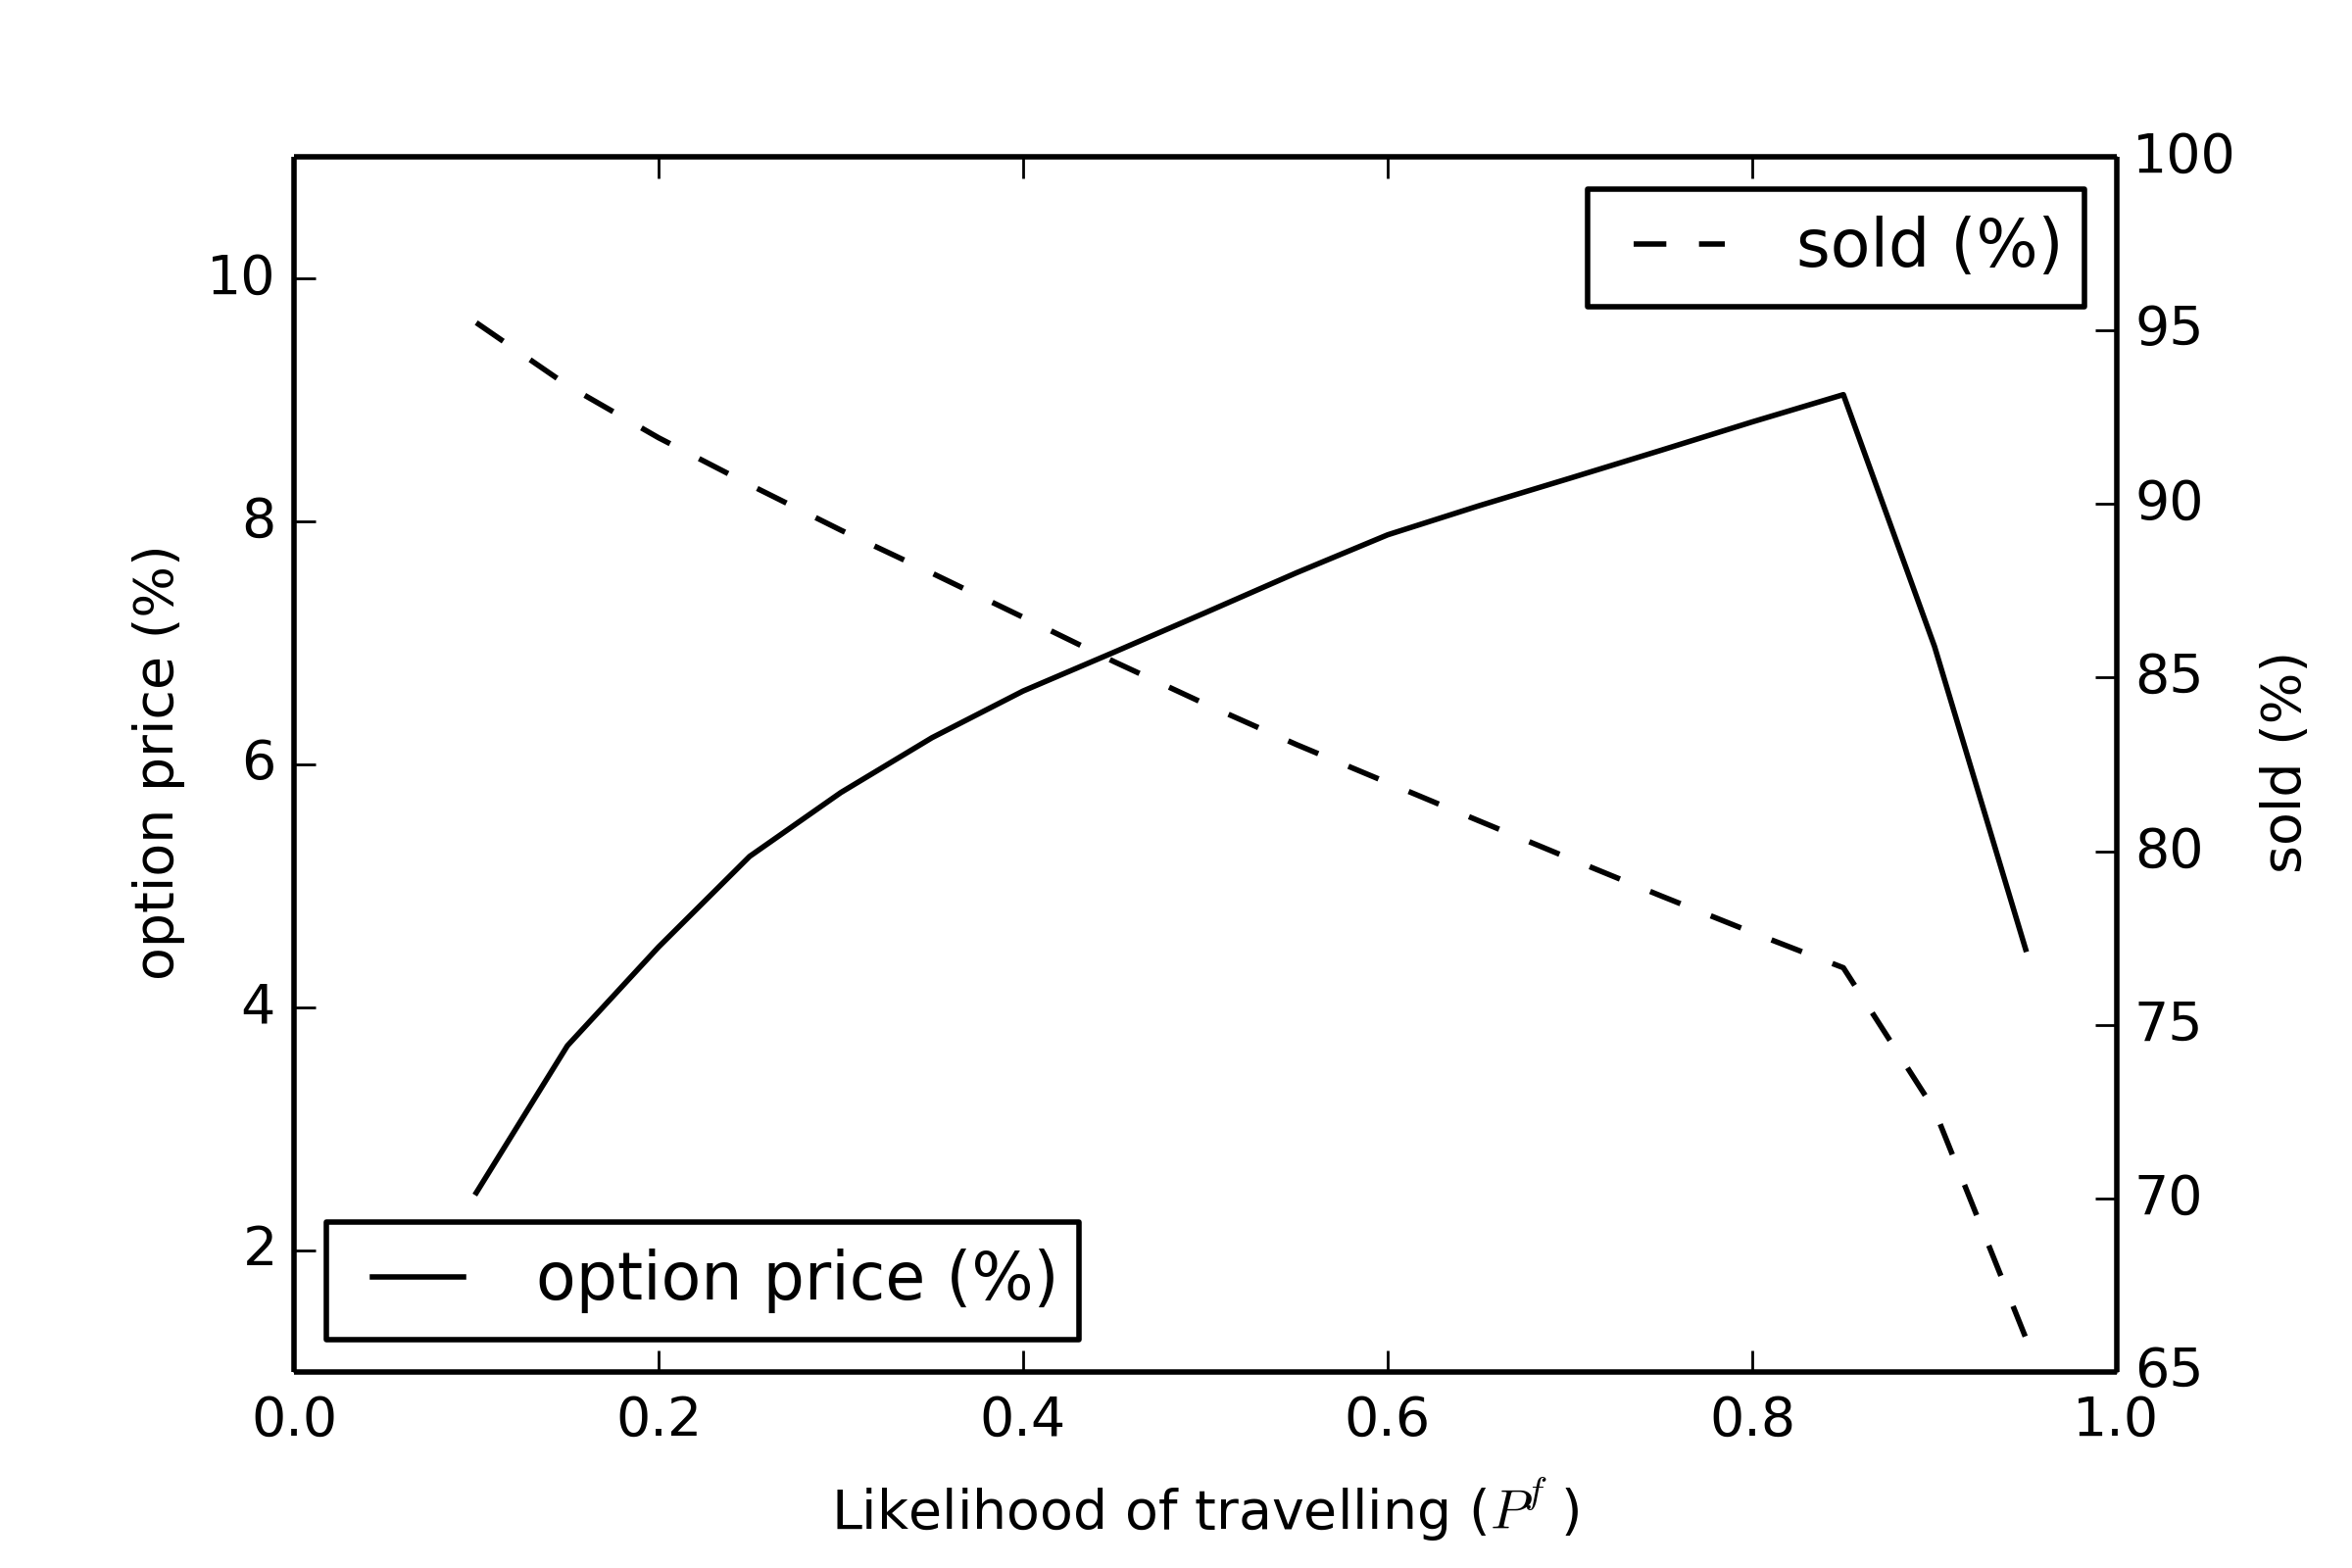
\includegraphics[width=0.8\textwidth]{figures/OptionPrice_Pf.png}
    \caption{Effect of likelihood of travelling ($P^f$)}
    \label{fig:OptionPrice_Pf}
\end{figure*}


The percentage of options sold also seems to be decreasing in this figure. This likely due to the all knowing assumption of the seller, in which he will always offer an option to a passenger that will not fly at maturity. Of course, when a passenger's probability of flying increases, he is also more likely to fly. Therefore the number of options sold will decrease.

At about the same level as the peak of the curve of the relative option price there seems to be an acceleration of the decrease in options sold. This is due to turning point of passengers buying the flights immediately as described previously.

The passenger's likelihood of travelling also seems to be of big influence on the results gained from the simulation. This was already expected due to the theoretical formulation described in \typenameref{chap:Methodology}. In the further analyses, the level of $P^f$ will be initially set at 0.85, as this seems to be the optimum for this parameter. \todo[However, to see whether the sensitivity is diferent in other simulations, this parameter will also be tested for different levels in the other models.]{here}


\subsection{Conclusion}
The simulation and sensitivity analysis ran in the previous section provide interesing results in this theoretical simulation model. The outcomes also provide insight into the first research question:

\begin{quote}\emph{Is it sustainable for an external company without capacity information or seat reservation capabilities to set the price of airfare~lock-in~products at a level that the customer accepts?}\end{quote}

While it is a theoretical model with many simplifications and assumptions of a real world setting, it does show it is possible to create a option valuation model that can offer airfare~lock-in products in a sustainable way. It does so by forecasting future airfares in an accurate way, and uses the uncertainties available at the customer's side to create profits in the model. The model thus shows that when a company is able to replicate such properties in a real setting, it can sell options to customers in a sustainable manner.

However, some assumptions and parameters of the model are unlikely to occur in a realistic setting. For example, a forecasting system which predicts flight ticket movements with a 100~percent accuracy is close to impossible. Therefore, this research will focus on two more option valuation methods: the Black--Scholes model which assumes random price fluctuations, and the Monte~Carlo simulation which uses empirically obtained data to make its predictions. The next two sections will analyse the results gained in these models.


\todo{RQ 2}

\section{Simulation 2: based upon Black--Scholes}
The second simulation model used in this research is based upon the Black--Scholes model. This model is the first of the two models which are practically implementable in a real world setting. By analyzing the results acquired from running this simulation, one can conclude whether it might be possible for an external seller to sell airfare~lock-in products in a sustainable way.

The Black--Scholes model makes the assumption that the returns or fluctuations of the underlying asset are log-normally distributed. When fluctuations of ticket prices are totally random and unpredictable, this model thus should be the most optimal option price setter possible. However, as shown in \autoref{subsec:DescriptiveAnalysisOfFareChanges}, it does not seem that the price fluctuations of flight tickets follow such a distribution. Therefore it is not expected that this model will perform very well.

This model thus makes its predictions based on the Black--Scholes equation found in \autoref{app:AdaptedBlackScholesFormula}. This formula uses the volatility of the stock to create its forecasts. This volatility is calculated on the historical price changes as seen in the training dataset. The equation used for the computation of the volatility is defined as:
$$\sigma_d = \sqrt{\frac{i}{N-1}\sum_{i=1}^N(x_i - \bar{x})^2} $$

This calculates the daily volatility of the price changes. To calculate the annual volatility of the fares, the following equation is used:
$$\sigma_a = \sigma_d \times \sqrt{365} $$

Next to this volatility, $\sigma_a$, the Black--Scholes equation also makes use of a risk free rate. In this research the value of the 10~year United States Governmental Bonds has been used to represent this value. This value is 2.57\,\% at the time of writing.

This simulation model is based upon the first simulation which represented the all knowing seller. A few modifications have been made to the parameters and assumptions to align with the theory behind this simulation model.

First, the seller's forecasting technique is no longer based upon foreknowledge, but uses the training set as its historical input for creating forecasts. By doing so, this model will practically implementable in a real world setting.

Second, the likelihood of flying has been altered to represent the value that was yielded from the sensitivity analysis. The parameter $P^f$ is thus set at the level of 0.85.

The rest of the parameters have been left similar to the configuration of the model for the all knowing seller. A summary can be found in \autoref{tbl:ParameterConfigBlackScholes}.


\begin{table}
\begin{center}
\begin{tabular}{l l c r}
    \toprule
    \#  & Parameter  &  Symbol  &  Level \\
    \midrule
    1  &  option's days till maturity  &  $m$  & 3~days \\
    2  &  option's strike price  &  $p_S$  &  $p_I$  \\
    3  &  seller's forecasting technique  &  ~  & foreknowledge \\
    4  &  passenger's risk parameter  &  $\mbox{RP}$  &  0.1 \\ 
    5  &  passenger's forecasting technique  &  ~  &  historical data \\
    6  &  passenger's likelihood of travelling  &  $P^f$  &  0.85 \\
    7  &  arrival rate of passengers  &  ~  &  $(42 - m)$ per flight \\
    8  &  simulation's number of trials  &  $N$  &  150 \\
    \bottomrule
\end{tabular}
\caption{Parameters for the model based upon Black--Scholes}
\label{tbl:ParameterConfigBlackScholes}
\end{center}
\end{table}


In the simulation with the all knowing seller with foresight, three assumptions were made. One of this assumptions has been released. This assumption involves the knowledge of the seller regarding whether the passenger will exercise its option (i.e., assumption number 2). In this simulation model, the seller thus no longer has the ability to know whether the customer will exercise his option at the date of maturity. Therefore, the writer now has to estimate his minimum Willingness To Accept upon the passenger's likelihood of flying, $P^f$. The other two assumptions are still applicable to this model:
\begin{compactenum}
\item the option's maximum price shall not exceed 15~percent of the current ticket price;
\item the seller knows the exact level of the customer's Willingness to Pay.
\end{compactenum}

This second simulation model is thus used to see whether a practically feasible technique might work. Instead of the theoretically optimal, this simulation will yield figures which a seller in a real world setting might have encountered. To test its performance, a comparison is made with a base case. This base case is the all knowing seller with foreknowledge in which the parameters $m$, $p_S$, $\mbox{RP}$, $P^f$, $N$, and the arrival rate have been set equal to this model.


\subsection{Analysis of the results}
\label{subsec:AnalysisOfBS}
The simulation was first run by categorizing per route and using the parameters and assumptions described in previous section. The outcomes of this simulation run can be found in \autoref{tbl:resultsBS} of \autoref{app:SimulationResultsBS}.

One should immediately notice that on most of the routes, the profits on option prices are negative (i.e., losses). Some routes, however, seem to make large returns on the airfare~lock-in products. These routes --- like JFK to CDG, JFK to LHR, LHR to JFK, and LHR to LAX -- also seem to be the routes with a very high standard deviation (See \autoref{tbl:DescriptiveAnalysisEntireDataset}). The flights with a much lower standard deviation seem to perform much worse. The correlation between the absolute option profits and the standard deviation in flight prices is illustrated in \autoref{fig:corrProfits_STD_BS}. Pearson's correlation test shows a coefficient of $\rho = 0.9295$, which is significant at a p-value of $< 0.001$.




\begin{figure*}
    \centering
    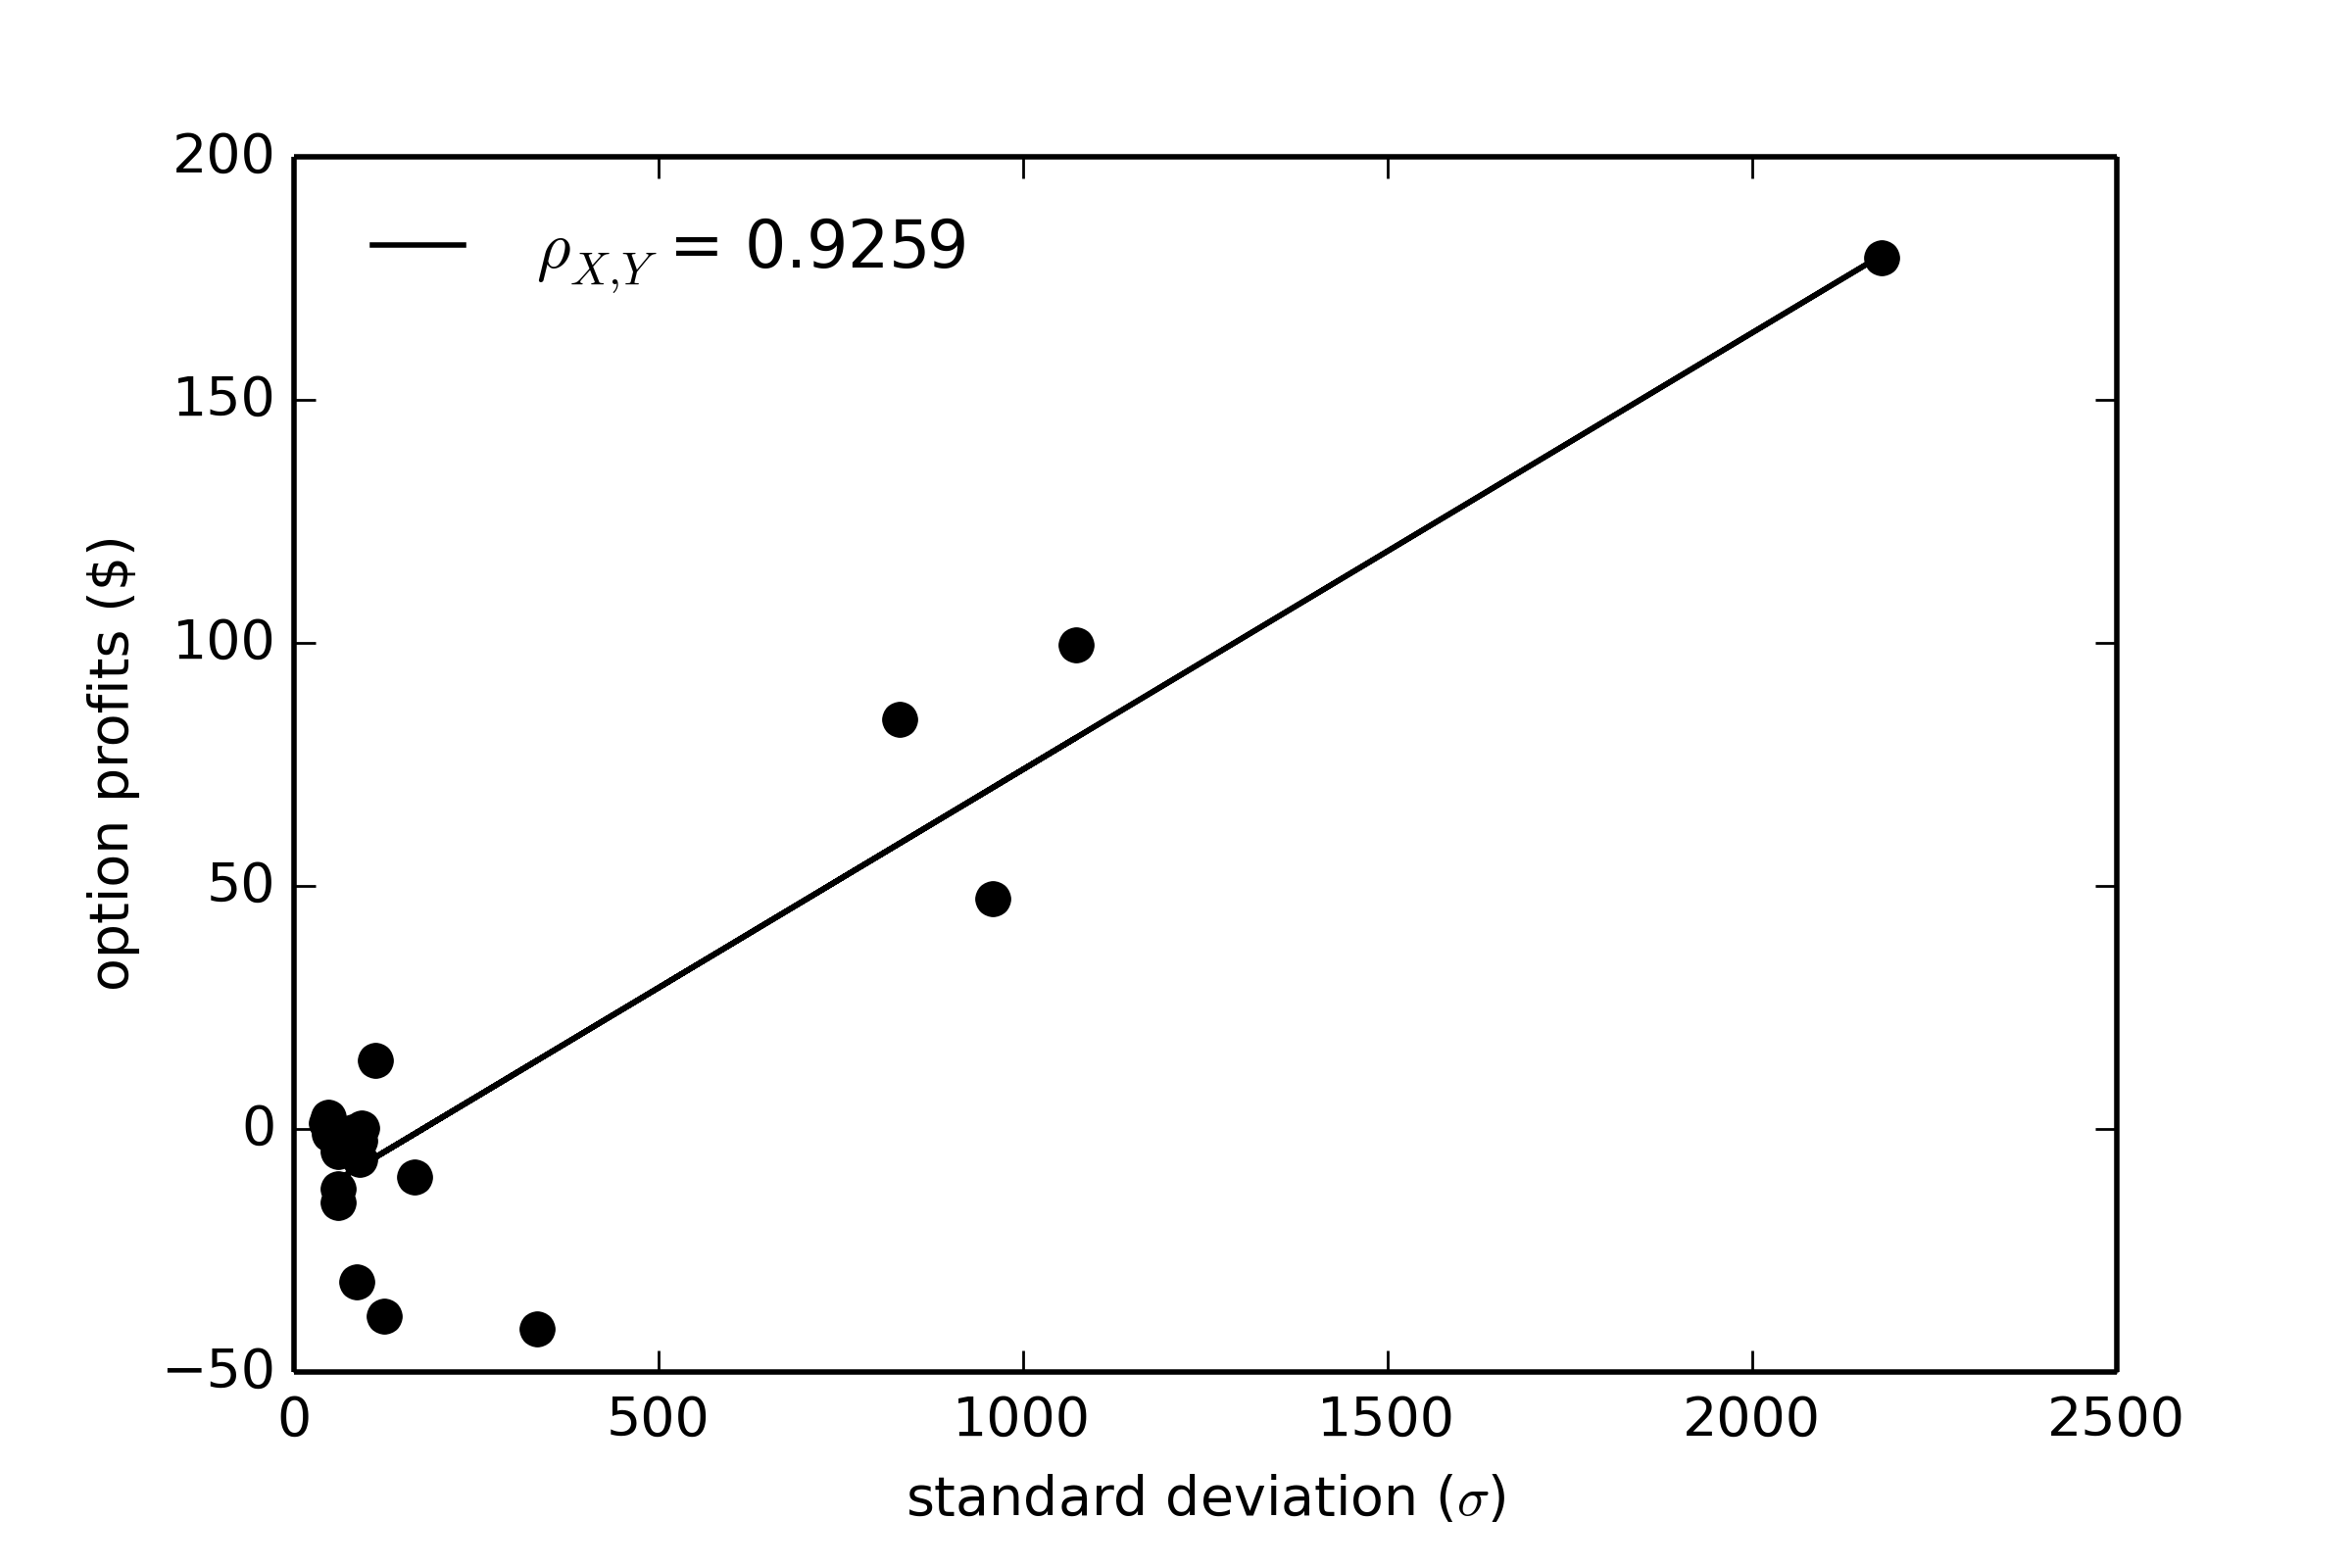
\includegraphics[width=0.8\textwidth]{figures/correlation_optionProfits_STD_BS}
    \caption{Correlation between option profits and standard deviation}
    \label{fig:corrProfits_STD_BS}
\end{figure*}

According to the analysis, there thus seems to be a strong possitive correlation present between the option profits acquired via the Black--Scholes model, and the standard deviation of the flight. This is likely due to the possibility that the Black--Scholes model underestimates the price fluctuations for routes with a low volatility. The model therefore offers options to customers with a too low WTP, and makes large losses on these customers. On the other hand, the writers sets his Willingness To Accept for routes with a exterme standard deviation to a much higher level. In that scenario, only customers with a high WTP will accept the offer, which thus results in a much higher profit. 

To test whether the forecasting accuracy of the option seller also had something to do with the profitability of certain routes, another correlation analysis was performed. In this case, Pearson's correlation coefficient was calculated to obtain the $\rho_{X,Y}$ between the writer's mean absolute percentage error ($\mbox{MAPE}$), and the absolute mean profits per option. However, as can be concluded from the results shown in \autoref{tbl:pearsonProfitsMAPE}, there seems to be no significant correlation between the two variables.

\begin{table}
\centering
\begin{tabular}{l c c}
\toprule
~  &  $\rho_{X,Y}$  &  p-value   \\
\midrule
Pearson's correlation test &  0.1774  &  0.43  \\
\bottomrule
\end{tabular}
\caption{Correlation of option profits and passenger's $\mbox{MAPE}$}
\label{tbl:pearsonProfitsMAPE}
\end{table}


To evaluate the performance of the simulation, the mean absolute profits per sold option of the model are compared with the base case's profits. As described before, this base case is the all knowing option seller with foreknowledge. All the other parameters and assumptions are aligned with the current model to get results on the most optimal prices in the same setting. The relative base profit in this research is defined as:
$$R_p =  \frac{M_p}{B_p}$$

Where $R_p$ is the relative profit, $M_p$ is the model profit of the current simulation, and $B_p$ is the base profit. \autoref{tbl:resultsBSrelative} gives an overview of the profits per option relative to the base case. Negative percentages correspond to losses.


\begin{table}
    \begin{center}
        \begin{tabular}{l l c| l r c}
            \toprule
             \multicolumn{2}{c}{Airport}  &  $R_p$   & \multicolumn{2}{c}{Airport}  &  $R_p$ \\
from  &  to  &  (\%) &  from  &  to  & (\%) \\
\midrule
AMS  &  CDG  &  -13.08  & JFK  &  CDG  &  94.62  \\
~    &  DXB  &  -38.29  & ~    &  LHR  &  46.96  \\
~    &  JFK  &  -147.49 & LAX  &  LAS  &  -20.01 \\
~    &  LHR  &  -5.60   & ~    &  SFO  &  64.60  \\ 
ATL  &  LAX  &  -31.87  & LHR  &  AMS  &   3.05  \\
~    &  MCO  &  16.91   & ~    &  JFK  &  99.18  \\
CDG  &  AMS  &  -8.69   & ~    &  LAX  &  78.34  \\
~    &  LHR  &  -41.63  & ~    &  MAD  &  -85.73 \\
DEN  &  FLL  &  -163.04 & ORD  &  BOS  &  -89.16 \\
~    &  PHX  &  13.01   & ~    &  LGA  &  -6.33  \\
DFW  &  LAX  &  -197.79 \\
~    &  SFO  &  -143.58 \\
            \bottomrule
        \end{tabular}
        \caption{Profits per sold option relative to base case}
        \label{tbl:resultsBSrelative}
    \end{center}
\end{table}


As stated before, the Black--Scholes model seems to underperform the optimal model significantly for most routes. The largest part of flights even shows a negative return. However, some routes' predictions using the Black--Scholes equation approach the optimal airfare~lock-in price. As concluded from prior analysis, this has to do with the associated high standard deviation for those specific routes. Furthermore, these routes probably approach the 15~percent maximum option price level. So while the actual optimal option price might differ, it is set to this assumed maximum WTP of the customer.


